\documentclass[12pt]{article}
\usepackage{graphicx}
\usepackage{url}
\usepackage[utf8]{inputenc}
\usepackage[brazil]{babel}
\usepackage{amsmath}
\usepackage{amsfonts}
\usepackage{booktabs}

\sloppy

\begin{document}
	
	\title{Análise Comparativa de Algoritmos de Ordenação}
	\author{David Nunes Ribeiro}
	\maketitle
	
	\begin{abstract}
		Este trabalho apresenta uma análise comparativa de desempenho dos algoritmos de ordenação Selection Sort, Insertion Sort, Bubble Sort e Quicksort. Foram avaliados o tempo de execução, o número de comparações e o número de movimentações para vetores de tamanhos 100, 1000, 10000 e 100000. Os resultados mostram que o Quicksort é significativamente mais eficiente para entradas maiores, enquanto os outros algoritmos apresentam desempenho quadrático. Este relatório discute os resultados e explica as diferenças de desempenho com base nas características de cada algoritmo.
	\end{abstract}
	
	\section{Introdução}
	A ordenação é uma operação fundamental em ciência da computação, com aplicações em diversas áreas. Este trabalho compara quatro algoritmos de ordenação clássicos: Selection Sort, Insertion Sort, Bubble Sort e Quicksort. Cada algoritmo foi implementado em Java, e seu desempenho foi medido em termos de tempo de execução, número de comparações e número de movimentações para vetores de números inteiros aleatórios com tamanhos 100, 1000, 10000 e 100000. Os resultados foram visualizados em gráficos gerados com a biblioteca matplotlib e analisados criticamente.
	
	\section{Metodologia}
	Os algoritmos foram implementados em Java, com contadores para comparações e movimentações. Para cada tamanho de entrada (100, 1000, 10000, 100000), foi gerado um vetor de números inteiros aleatórios. Cada algoritmo foi executado em uma cópia do vetor original para garantir condições idênticas. O tempo de execução foi medido em milissegundos usando \texttt{System.currentTimeMillis()}. Os resultados foram salvos em um arquivo CSV e usados para gerar gráficos com matplotlib. A análise considera a complexidade teórica e os resultados empíricos.
	
	\section{Resultados}
	Os resultados são apresentados em três gráficos: tempo de execução, número de comparações e número de movimentações.
	
	\begin{figure}[h]
		\centering
		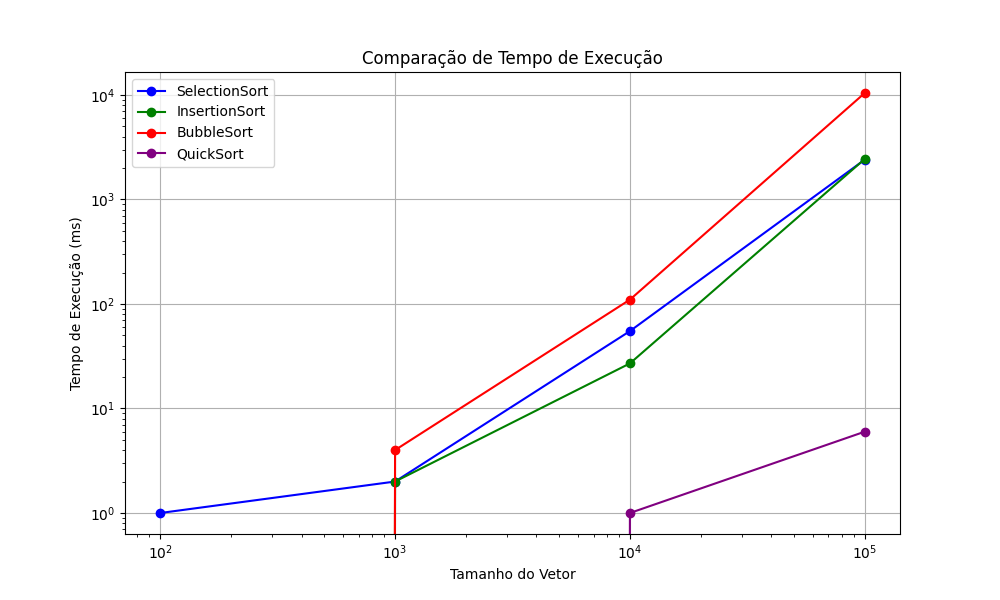
\includegraphics[width=0.8\textwidth]{tempo_execucao.png}
		\caption{Tempo de execução dos algoritmos para diferentes tamanhos de entrada.}
		\label{fig:tempo}
	\end{figure}
	
	\begin{figure}[h]
		\centering
		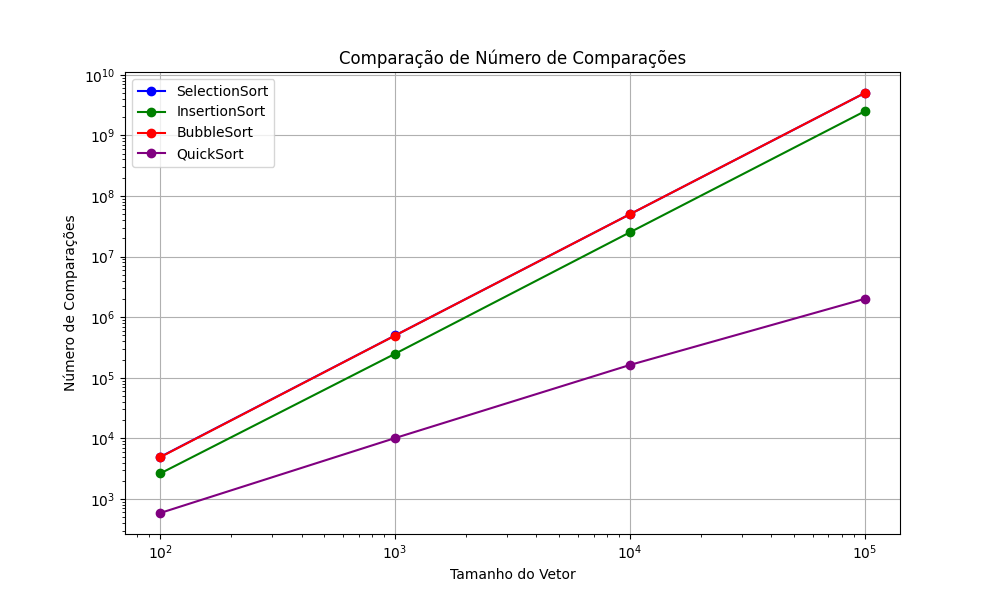
\includegraphics[width=0.8\textwidth]{comparacoes.png}
		\caption{Número de comparações realizadas pelos algoritmos.}
		\label{fig:comparacoes}
	\end{figure}
	
	\begin{figure}[h]
		\centering
		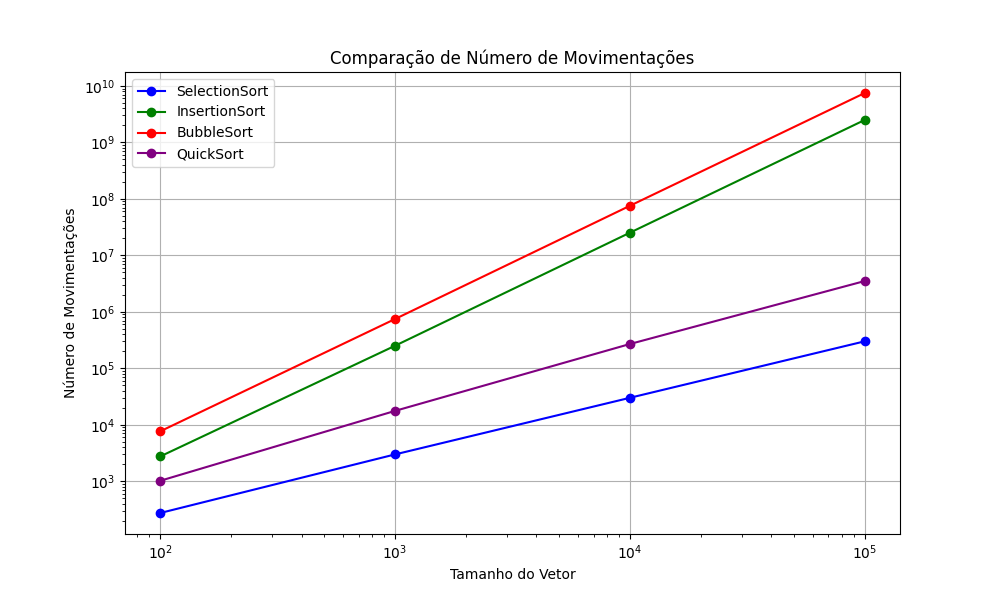
\includegraphics[width=0.8\textwidth]{movimentacoes.png}
		\caption{Número de movimentações realizadas pelos algoritmos.}
		\label{fig:movimentacoes}
	\end{figure}
	
	\subsection{Tempo de Execução}
	Conforme mostrado na Figura~\ref{fig:tempo}, o Quicksort apresenta o melhor desempenho, com tempos de execução significativamente menores para entradas maiores. Para $n=100000$, o Quicksort é ordens de magnitude mais rápido que os outros algoritmos. Selection Sort, Insertion Sort e Bubble Sort exibem comportamento quadrático, com tempos de execução crescendo rapidamente com o aumento de $n$. O Insertion Sort é ligeiramente mais rápido que os outros dois para entradas menores devido a menos movimentações.
	
	\subsection{Número de Comparações}
	A Figura~\ref{fig:comparacoes} mostra que o Quicksort realiza menos comparações, com uma complexidade média de $O(n \log n)$. Selection Sort e Bubble Sort realizam aproximadamente $n^2/2$ comparações, enquanto o Insertion Sort pode realizar menos comparações em vetores parcialmente ordenados, mas mantém $O(n^2)$ no caso médio. Para $n=100000$, o Quicksort realiza cerca de 2 milhões de comparações, contra bilhões para os outros algoritmos.
	
	\subsection{Número de Movimentações}
	Na Figura~\ref{fig:movimentacoes}, observa-se que o Insertion Sort realiza menos movimentações que Selection Sort e Bubble Sort, especialmente para entradas menores, devido à sua estratégia de inserção. O Quicksort, embora eficiente em comparações, realiza mais movimentações que o Insertion Sort em alguns casos, mas seu desempenho geral é superior devido à menor complexidade. Selection Sort e Bubble Sort apresentam $O(n^2)$ movimentações, tornando-os ineficientes para grandes entradas.
	
	\section{Análise Crítica}
	O Quicksort é o algoritmo mais eficiente para entradas maiores devido à sua complexidade $O(n \log n)$ no caso médio. Sua estratégia de divisão e conquista reduz significativamente o número de operações. Para entradas pequenas ($n=100$), a diferença de desempenho é menos pronunciada, e o Insertion Sort pode ser competitivo devido à sua simplicidade e menor número de movimentações.
	
	Selection Sort e Bubble Sort são ineficientes para grandes entradas devido à complexidade $O(n^2)$. O Bubble Sort é particularmente ruim, pois realiza trocas desnecessárias mesmo em vetores quase ordenados. O Insertion Sort é mais eficiente que os dois em vetores parcialmente ordenados, mas ainda não compete com o Quicksort em grandes escalas.
	
	As diferenças de desempenho decorrem das estratégias dos algoritmos. Quicksort reduz o problema em subproblemas menores, enquanto os outros algoritmos processam o vetor inteiro repetidamente. Para aplicações práticas, o Quicksort é preferível, exceto em casos específicos, como vetores muito pequenos ou quase ordenados, onde o Insertion Sort pode ser mais adequado.
	
	\section{Conclusão}
	A análise confirma que o Quicksort é o algoritmo mais eficiente para ordenação de vetores grandes, com tempos de execução, comparações e movimentações significativamente menores. Selection Sort, Insertion Sort e Bubble Sort são adequados apenas para entradas pequenas ou casos específicos. Os resultados reforçam a importância de escolher o algoritmo apropriado com base no tamanho da entrada e nas características dos dados.
	
\end{document}